\section{问题一：常物性下预热阶段的热-质输运模型与半解析校核}

\subsection{本问模型}

本问沿用公共模型一章的式~\eqref{eq:energy}--\eqref{eq:ic}，物性取式~\eqref{eq:prop_app2}。
由于 $\rho$、$c_p$、$k$ 均为常数，式~\eqref{eq:energy} 化为线性热传导方程

\begin{equation}\label{eq:p1_heat}
\frac{\partial T}{\partial t}=\alpha\,\frac{1}{r}\frac{\partial}{\partial r}\!\left(r\,\frac{\partial T}{\partial r}\right),
\qquad \alpha=\frac{k}{\rho c_p}=1.6886\times10^{-7}~\mathrm{m^2/s},
\end{equation}

而水分方程保留非线性

\begin{equation}\label{eq:p1_mass}
\frac{\partial C}{\partial t}=\frac{1}{r}\frac{\partial}{\partial r}\!\left(r\,D(C)\,\frac{\partial C}{\partial r}\right),
\qquad D(C)=7\times10^{-9}\,\mathrm{e}^{-0.89/C}.
\end{equation}

式~\eqref{eq:p1_heat} 不含 $C$、式~\eqref{eq:p1_mass} 不含 $T$，两者在题给物性下完全解耦，
仅共享几何域和环境时间轴。
这一解耦不是人为简化，而是附录 2 物性关系的直接后果，也正是本问可以引入独立数学基准的原因。
初始含水率下 $D(C_0)=4.94\times10^{-9}$~m$^2$/s，与 $\alpha$ 相差 $34$ 倍，
预示两个场在同一时间窗内的推进深度将有量级差别。

时间步长取 $\Delta t=1$~s，推进至 $1800$~s。

\subsection{温度场与含水率场的结果}

按题目要求的时刻与位置整理结果，见表~\ref{tab:p1_T} 与表~\ref{tab:p1_C}。

\begin{table}[H]
\centering
\caption{预热阶段药材内部温度（$^\circ$C）}\label{tab:p1_T}
\begin{tabular}{cccccc}
\toprule
时间 (s) $\backslash$ 距中心距离 (cm) & 0 & 0.5 & 1 & 1.5 & 2 \\
\midrule
100  & 28.0001 & 28.0004 & 28.0043 & 28.0332 & 28.1803 \\
300  & 28.0416 & 28.0643 & 28.1523 & 28.3690 & 28.8493 \\
600  & 28.4550 & 28.5377 & 28.8054 & 29.3170 & 30.1659 \\
900  & 29.3263 & 29.4601 & 29.8770 & 30.6173 & 31.7311 \\
1200 & 30.5446 & 30.7115 & 31.2239 & 32.1138 & 33.4285 \\
1500 & 31.9974 & 32.1883 & 32.7673 & 33.7472 & 35.1209 \\
1800 & 33.5765 & 33.7731 & 34.3652 & 35.3630 & 36.7862 \\
\bottomrule
\end{tabular}
\end{table}

\begin{table}[H]
\centering
\caption{预热阶段药材内部水分浓度（kg/kg）}\label{tab:p1_C}
\begin{tabular}{cccccc}
\toprule
时间 (s) $\backslash$ 距中心距离 (cm) & 0 & 0.5 & 1 & 1.5 & 2 \\
\midrule
100  & 2.5500 & 2.5500 & 2.5500 & 2.5500 & 2.2555 \\
300  & 2.5500 & 2.5500 & 2.5500 & 2.5490 & 2.0545 \\
600  & 2.5500 & 2.5500 & 2.5500 & 2.5349 & 1.8789 \\
900  & 2.5500 & 2.5500 & 2.5496 & 2.5044 & 1.7560 \\
1200 & 2.5500 & 2.5500 & 2.5481 & 2.4646 & 1.6595 \\
1500 & 2.5500 & 2.5499 & 2.5444 & 2.4208 & 1.5794 \\
1800 & 2.5500 & 2.5497 & 2.5381 & 2.3757 & 1.5108 \\
\bottomrule
\end{tabular}
\end{table}

两表呈现的格局截然不同。温度在 $1800$~s 内各位置都有明显上升，中心由 $28~^\circ$C 升至
$33.5765~^\circ$C、表面升至 $36.7862~^\circ$C，且同一时刻始终满足表面高于中心的单调序；
含水率则只有表面有大幅下降（由 $2.55$ 降至 $1.5108$~kg/kg），$r=1.5$~cm 处降幅
$0.174$~kg/kg，而中心处四位小数下仍显示为 $2.5500$~kg/kg。这一对照即
式~\eqref{eq:p1_heat} 与式~\eqref{eq:p1_mass} 中输运系数相差 $34$ 倍的直接体现。
表面含水率在前 $100$~s 内即降至 $2.2555$~kg/kg，说明表面失水几乎从加热一开始就发生，
但它并未立即传递到内部。

温度剖面与含水率剖面的空间形态见图~\ref{fig:q1_profiles}。

\begin{figure}[H]
  \centering
  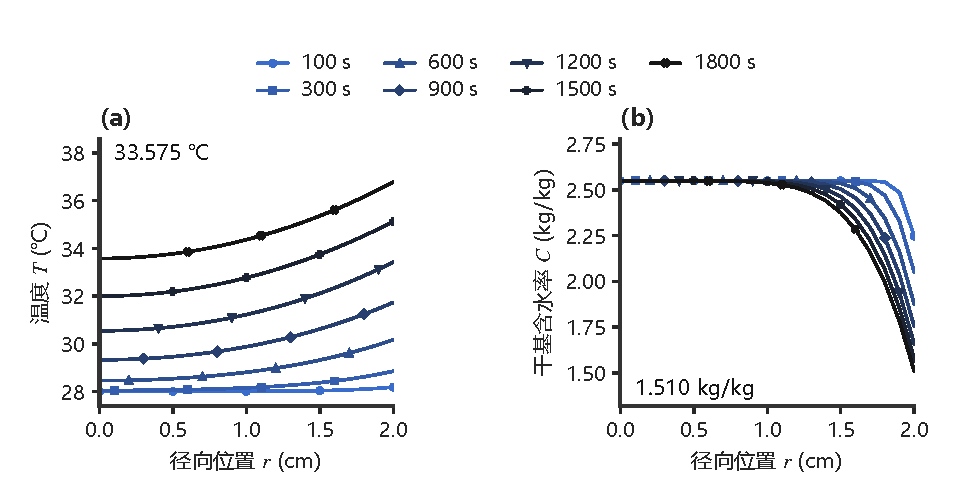
\includegraphics[width=0.9\textwidth,height=0.8\textheight,keepaspectratio]{../figures/fig_q1_profiles.pdf}
  \caption{问题一温度与含水率的径向剖面}
  \label{fig:q1_profiles}
\end{figure}

图中两个面板共用一条时刻色带。温度剖面自初值起整体抬升，各时刻都保持表面高、中心低的
单调形状，且梯度在整个半径上都不为零，说明热扰动已穿透全域。含水率剖面则始终贴合初值线，
仅在 $r\gtrsim1.5$~cm 的外层出现可见弯折，中心处相对初值仅降低
$1.0\times10^{-5}$~kg/kg。若把两个面板的可见变化区厚度相比，水分的影响深度不足半径的四分之一。

中心与表面两个测点的时程对照进一步给出量化的层级关系，见图~\ref{fig:q1_center_surface}。

\begin{figure}[H]
  \centering
  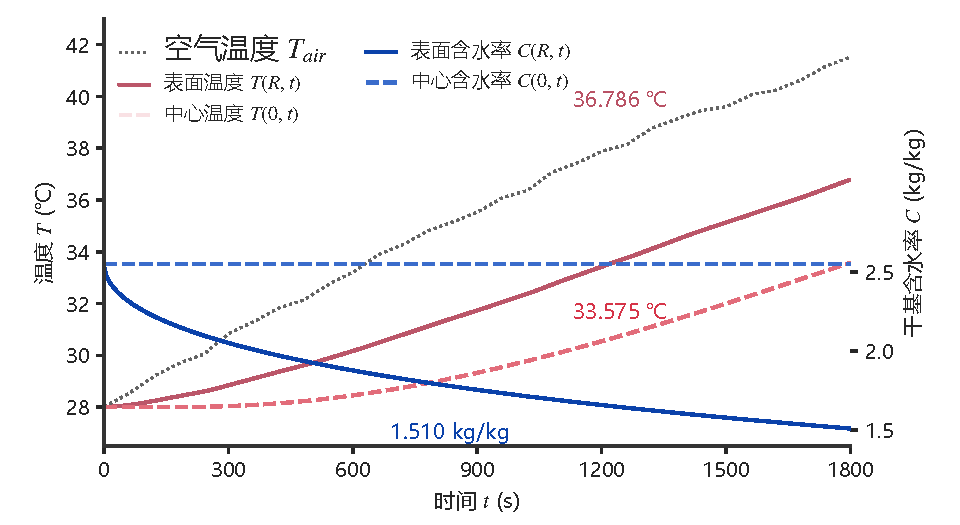
\includegraphics[width=0.9\textwidth,height=0.8\textheight,keepaspectratio]{../figures/fig_q1_center_surface.pdf}
  \caption{问题一中心与表面测点的时程对照}
  \label{fig:q1_center_surface}
\end{figure}

左轴三条温度曲线全程保持空气高于表面、表面高于中心的次序，这与第三类边界的方向一致：
热流始终由空气流向药材，且表面必须低于空气温度才能维持正向换热。若表面温度追平空气温度，
则说明表面阻力被忽略，与 $Bi_h=1.389$ 的估计矛盾。右轴的中心含水率曲线在
$1800$~s 内近乎水平（终值 $2.54999$~kg/kg），可以读出中心水分在预热阶段基本未被动用。

两个场的渗透深度差异在时空分布上更为直观，见图~\ref{fig:q1_spacetime}。

\begin{figure}[H]
  \centering
  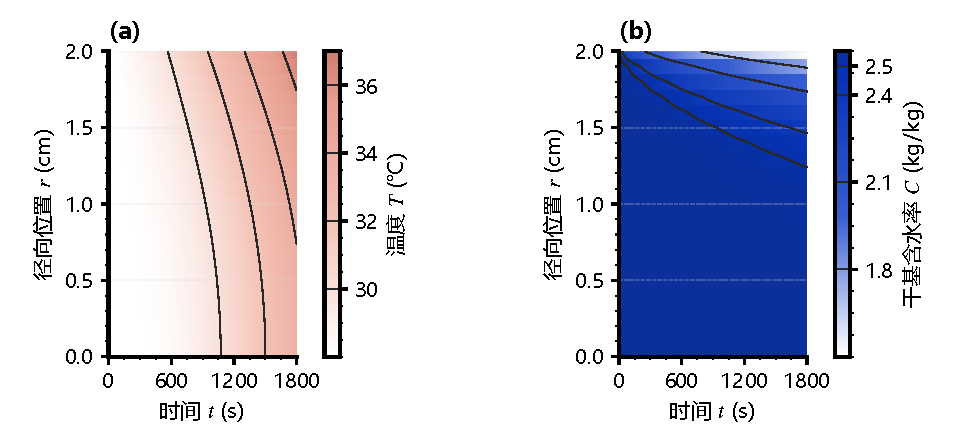
\includegraphics[width=0.9\textwidth,height=0.8\textheight,keepaspectratio]{../figures/fig_q1_spacetime.pdf}
  \caption{问题一温度场与含水率场的时空分布}
  \label{fig:q1_spacetime}
\end{figure}

温度场的色阶变化在 $1800$~s 内已铺满整个纵向坐标，含水率场的可见变化则被压在图幅顶部一条
窄带内：$r=1.5$~cm 处降幅 $0.174$~kg/kg，到 $r=0.7$~cm 处已不足 $1.5\times10^{-3}$~kg/kg，
两个位置相距仅 $0.8$~cm 而降幅差两个数量级。由此可以给出预热阶段的物理图景：
热量先行铺满全域并把药材整体加热，水分迁移则从表面开始逐层向内推进，
中心水分要到进入恒温干燥阶段之后才会明显下降。这一时标分离也解释了为何题目把
预热阶段与整个烘干过程分开设问——两个阶段的控制机制并不相同。

\subsection{半解析级数解的独立校核}

式~\eqref{eq:p1_heat} 是常系数线性方程，配合第三类边界与均匀初值，可用分离变量法求解。
对阶跃型环境温度，特征值 $\lambda_n$ 由

\begin{equation}\label{eq:bessel_eig}
\lambda_n J_1(\lambda_n)=Bi_h\,J_0(\lambda_n),\qquad Bi_h=\frac{hR}{k}=1.389
\end{equation}

确定，$J_0$、$J_1$ 为零阶与一阶第一类 Bessel 函数，该本征关系是无限长圆柱对流换热问题的
经典结果\upcite{Guellal2009}。实际环境温度并非阶跃而是随时间变化，
故按 Duhamel 原理把 $T_{\rm air}(t)$ 的分段线性时程分解为一系列阶跃响应的叠加，得到

\begin{equation}\label{eq:duhamel}
T(r,t)=T_{\rm air}(0)+\int_0^t \frac{\mathrm{d}T_{\rm air}(\tau)}{\mathrm{d}\tau}\,
\Phi\!\left(r,\,t-\tau\right)\mathrm{d}\tau,\qquad
\Phi(r,s)=1-\sum_{n=1}^{\infty} A_n\,J_0\!\left(\lambda_n \frac{r}{R}\right)
\mathrm{e}^{-\alpha\lambda_n^2 s/R^2},
\end{equation}

其中 $A_n$ 为由初值与正交性确定的展开系数，$\Phi$ 为单位阶跃响应。
式~\eqref{eq:duhamel} 的价值不在于它比数值解更精确，而在于它与
公共模型一章的离散格式完全无关：一条路径来自 Bessel 函数正交展开，另一条来自控制体通量平衡，
两者若吻合，则离散实现中的系数装配、边界处理与时间推进都得到了独立确认。
本文取前 $30$ 个特征根，并对分段线性的环境时程逐段精确叠加。
校核结果与网格、步长收敛证据一并给出，见图~\ref{fig:q1_validation}。

\begin{figure}[H]
  \centering
  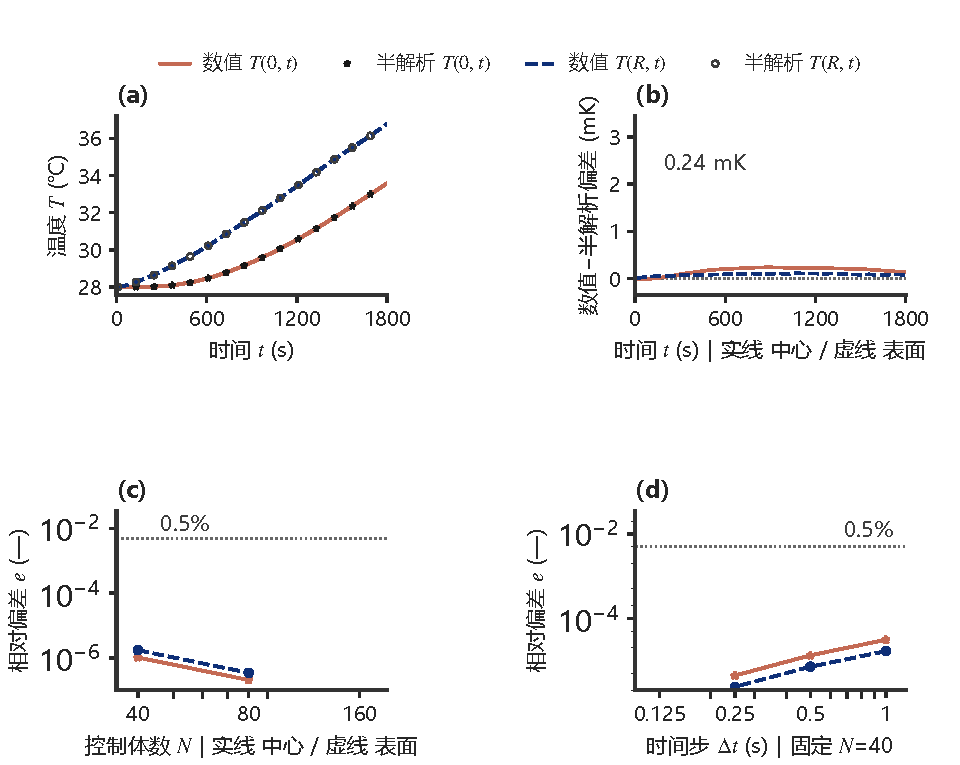
\includegraphics[width=0.9\textwidth,height=0.8\textheight,keepaspectratio]{../figures/fig_q1_validation.pdf}
  \caption{问题一数值解的四项校核证据}
  \label{fig:q1_validation}
\end{figure}

面板 (a) 中数值解与级数解的曲线逐点重合，面板 (b) 给出两者之差：中心与表面两条测点曲线
在 $1800$~s 全程内的最大偏差为 $1.97$~mK，相对于表面 $8.786~^\circ$C 的温升约为 $0.022\%$；
若只看末时刻沿半径的偏差，最大值为 $1.16$~mK 即 $0.0012~^\circ$C，约为温升的 $0.013\%$。
两个量级都与时间离散的截断误差相当，说明偏差来自 $\Delta t$ 而非模型实现有误。
面板 (c)(d) 为网格与时间步的加密收敛：交付网格 $N=40$ 相对 $N=160$ 参照解的偏差为
$e_T=2.76\times10^{-5}$、$e_C=3.04\times10^{-4}$，$\Delta t=1$~s 时 $e_T=2.45\times10^{-5}$，
均远低于图中标出的 $0.5\%$ 判据线。

需要说明的是，这一校核只覆盖温度场，因为水分方程含非线性扩散系数，不存在同类级数解。
水分场的可信度依靠守恒残差与网格收敛证据支撑，详见数值可信度一章。本问的质量收支相对残差为
$7.41\times10^{-16}$，已接近双精度浮点的机器精度，即离散格式在本问未引入可测的守恒破坏。

\subsection{完整场数据的交付}

按题目要求，$1800$~s 内每隔 $1$~s、距中心每隔 $0.1$~cm 的温度与含水率完整结果
以双表形式保存于结果文件中，数值保留四位小数。表格中的位置坐标由 $N=40$ 交付网格的结点值
按线性插值给出至题目要求的 $0.1$~cm 间隔。
